Psychological research has shown that people can learn from positive examples alone.\\
The \textbf{concept learning} can be thought as a binary classification. Let's define 
$f(x) = 1$ if $x$ is an example of the concept $\mathcal{C}$, $f(x) = 0$ otherwise.\\
Then the goal is to learn the indicator function $f$, which just defines the concept 
$\mathcal{C}$. The standard binary classification techniques require positive and 
negative examples. By contrast we will devise a way to learn from positive examples alone.
We can then propose a concept $\mathcal{C}$, for example "prime number", and then we look
into a randomly selected example $\mathcal{D} = \left\{x_{i}\right\}_{1\leq i \leq N}$
Some examples are more likely to belong to the concept $\mathcal{C}$.\\
$\ProbC{\mathcal{D}}{\tilde{x} \in \mathcal{C}}$ the probability that $\tilde{x} \in 
\mathcal{C}$ knowing that $\tilde{x}$ comes from $\mathcal{D}$. This probability is called
\textbf{posterior predictive distribution}.
Sometimes given $\mathcal{D}$ we have to find the concept $\mathcal{C}$ among what we call
the \textbf{hypothesis space} $\mathcal{H}$. 

\subsection{Likelihood}
Let's consider the set $\mathcal{D}=\{16, 8, 2, 64\}$ we would like to find the underneath
concept. Consider the following \emph{version space}, meaning a subset of $\mathcal{H}$
that is consistent with the data in $\mathcal{D}$: \{'$h_{x=2^{k}}$:powers of two',
$h_{x=2k}$'even numbers'\}.
We would like to avoid \emph{suspicious coincidences}.
We compute then the probability of independently sampling $N$ items (with replacement) 
from $h$ is given by: 
\begin{center}
    \encB{$\ProbC{h}{\mathcal{D}} = \left[ \dfrac{1}{size(h)} \right]^{N}$}. 
\end{center}

This crucial equation embodies what we size principle more commonly known as 
\textbf{Occam's razor}, it means that the model favors the simplest hypothesis consistent
with the data.

\subsection{Prior}
As prior we could choose a concept like "$h'$: powers of two except 32", meaning the prior
might be different than mine, this subjective aspect of Bayesian reasoning is the object
of lot of controversy. 

\subsection{posterior}
Posterior is by default the likelihood times the prior, normalized.

\begin{center}
    $\ProbC{\mathcal{D}}{h} = \dfrac{\ProbC{h}{\mathcal{D}}\Prob{h}}{
        \su{{h'\in\mathcal{H}}}{}\Prob{\mathcal{D}\cap h'}
    } 
    = \dfrac{ \frac{\Prob{h}\times\mathbbm{1}_{\{\mathcal{D}\in h\}}}{size(h)^{N}}}{
        \frac{\su{{h'\in\mathcal{H}}}{}\Prob{h'}\mathbbm{1}_{\{\mathcal{D} \in h'\}}}{size(h)^{N}}
    }$
\end{center}

As the MAP estimate can be written as:
\begin{align*}
    \hat{h}_{MAP} &= \argmax \ProbC{h}{\mathcal{D}}\times \Prob{h} \\
                  &= \argmax (\log(\ProbC{h}{\mathcal{D}}) + \log(\Prob{h})) \\
                  &= \argmax^{h} (N\times\log\left(\frac{1}{size(h)}\right) +
                  \log \left(\Prob{h}\right)
\end{align*}
We deduce that when we reach a sufficiently high level of observations the MAP converges
towards the \emph{maximum likelihood estimate (MLE)}.\\
Meaning, \tB{if we have enough data, the knowledge about data overwhelms the prior}.

\subsection{Posterior predictive distribution}
It is the way to test our posterior, meaning our belief state about the world. 
\begin{center}
    \encB{$\ProbC{\mathcal{D}}{\tilde{x}\in\mathcal{C}} = \su{h}{}
    \ProbC{\tilde{x}, h}{y=1}\ProbC{\mathcal{D}}{h}$}
\end{center}

\begin{figure}[H]
    \begin{center}
        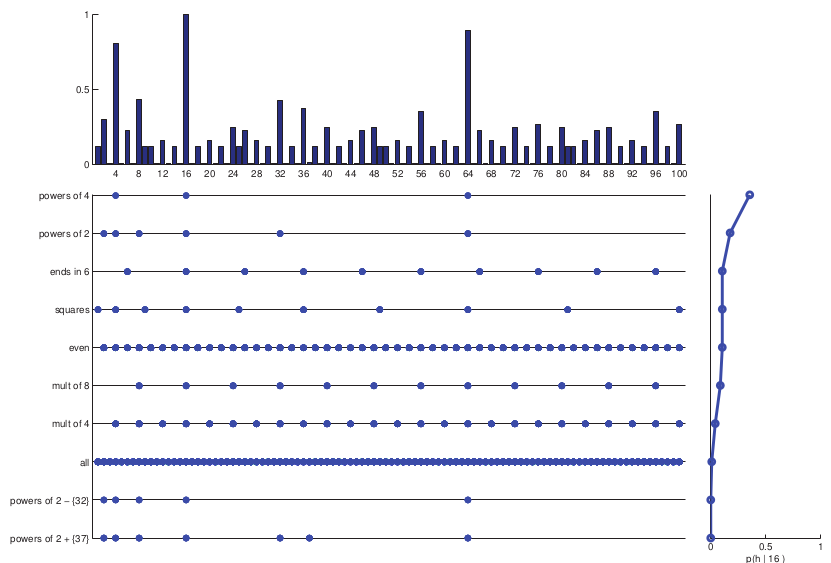
\includegraphics[width=\textwidth]{./chaps/31_sec/images/1_posterior_predictive_dist.png}
    \end{center}
    \caption{First assume $\mathcal{D}=\{16\}$\\ 
        Each row represents an hypothesis, the dots inside are the numbers consistent
        with this hypothesis. The graph on the right is the $\ProbC{\mathcal{D}}{h}$ the 
        weight given to the hypothesis $h$. Finally by taking a weighted sum of dots, 
        we get $\ProbC{\mathcal{D}}{\tilde{x}\in\mathcal{C}}$.}
    \label{fig:1_posterior_predictive_dist}
\end{figure}


